
%----------------------------------------------------------------------------------------
%   PACKAGES AND OTHER DOCUMENT CONFIGURATIONS
%----------------------------------------------------------------------------------------

% latexmk -pvc -pdf
\documentclass[12pt, a4paper]{report}
\usepackage[margin=2.5cm]{geometry}
\usepackage{titling}
\usepackage{titlesec}
\usepackage{amsmath,amsthm,amsfonts,amssymb}
\usepackage{mathtools}
\usepackage{braket}
\usepackage{dsfont}
\usepackage[font=scriptsize,labelfont=bf]{caption}
\usepackage[english]{babel}
\usepackage{graphicx}
\newenvironment{Figure}
    {\par\medskip\noindent\minipage{\linewidth}}
    {\endminipage\par\medskip}
\usepackage{tabularx}

% Colours:
\usepackage[table]{xcolor}
\definecolor{purple}{RGB}{117,77,226}

\usepackage[bookmarksopen,
  pagebackref,
  pdfpagelayout=TwoPageRight,
  colorlinks=true,
  urlcolor=purple,
  citecolor=purple,
  filecolor=purple,
  linkcolor=purple,
  urlcolor=purple,
  citecolor=purple,
  filecolor=purple,
  linkcolor=purple,
  linktocpage=true
  ]
{hyperref}

\titleformat{\chapter}[display]
  {\normalfont\bfseries}{}{0pt}{\Huge}

\newcommand\II{\(\mathcal{I}\)}
\newcommand\PT{\(\mathcal{PT}\)}
\newcommand\PP{\(\mathcal{P}\)}
\newcommand\TT{\(\mathcal{T}\)}
\newcommand\CPT{\(\mathcal{CPT}\)}
\newcommand\CC{\(\mathcal{C}\)}


\begin{document}
  \begin{center}
  \vspace{2cm}
  {\Huge \( \mathcal{PT} \)-symmetric quantum mechanics}\\
  \vspace{0.5cm}
  \textsc{Honours Literature review}\\
  \vspace{1cm}
  {\Large Ana Fabela Hinojosa\\Student ID: 27876594}\\
  \vspace{0.5cm}
  {\Large Supervisors:\\ Dr. Jesper Levinsen \\ Prof. Meera Parish\\\vspace{0.2cm}Dr. Brendan Mulkerin}\\
  \vspace{0.5cm}
  \textsc{School of Physics \& Astronomy}\\
  \vspace{0.5cm}
  \includegraphics[scale=0.2]{logo.jpg} \\ % University logo
  {11th November 2022}\\
  \vspace{3cm}
  \centering{\textbf{Abstract}}
 \\An underlying assumption of quantum theory is Hermiticity, which is a strict mathematical postulate that guarantees that predictions of observables satisfy specific physical criteria. All natural physical systems are in contact with an environment and in many cases this describes crucial features of said systems. Generally non-Hermitian quantum mechanics can describe systems which incorporate gain and loss from their environment and so physicists have developed an alternative postulate to Hermiticity known as \PT-symmetry. This postulate has shown to be consistent with all other aspects of the conventional theory. However a non-Hermitian \PT- symmetric quantum system has not yet been experimentally demonstrated.
  \end{center}


\tableofcontents

%%%%%%%%%%%%%%%%%%%%%%%%%%%%%%%%%%%%%%%%%%%%%%%%%%%%%%%%%%%%%%%%%%%%%%%%%%%%%%%%%%%%%%%%%%%%%%%
\chapter{Introduction}\label{Introduction}
In ``The principles of quantum mechanics", Paul Dirac advises us that``it is important to remember that science is concerned only with \textit{observable} things and that we can observe an object only by letting it interact with some outside influence"~\cite{POQM}. Observable interactions are measurable phenomena and overtime physicists have attempted to explain a number of experimental results with a set of ad-hoc rules that came to be known as the fundamental postulates of quantum theory. Nearly all these postulates are based in physical properties. For example, one postulate establishes that time evolution of a quantum system must be probability conserving. Another postulate requires that the energy spectrum of the system is bounded below so a lowest energy state can be measured. In quantum mechanics, the Hamiltonian operator $(\hat{H})$ encapsulates the total energy of a system. A system's energy spectrum is required to be bounded and real in order to be measurable. According to the fundamental postulates of the standard theory, if an operator $\hat{O}$ satisfies the mathematical property known as Hermiticity, then $\hat{O}$ will satisfy the other postulates of quantum theory.

If $\hat{O}$ is Hermitian then it has the property that its effect on the vectors of the Hilbert space in which $\hat{O}$ is defined is independent of the order in which $\hat{O}$ acts on said vectors~\cite{Jones-Smith}
\begin{equation}\label{eq:1.1}
\bra{\phi}\ket{\hat{O}\psi} = \bra{\hat{O}\phi}\ket{\psi},
\end{equation}
where $\ket{\hat{O}\psi} = \hat{O}\ket{\psi}$ and $\bra{\hat{O}\phi} = (\hat{O}\ket{\phi})^{\dagger}$
It may appear to the reader that there is no compelling reason to change this convenient mathematical assumption, since Hermiticity results in a ``correct" theory of quantum mechanics. But despite the correctness of Hermiticity, this postulate may have lead us to an overly restrictive quantum theory~\cite{MustaHbeHermitian}. The philosophically curious physicist will perhaps be persuaded to expand their mathematical toolbox by learning that not all non-Hermitian Hamiltonians describe physically invalid systems. Here it is relevant to quote the contrapositive of Gell-Mann's totalitarian principle: ``Anything not forbidden is compulsory"~\cite{MGM}. This means that if there exists valid alternative non-Hermitian quantum theory then we must use it to study this class of Hamiltonians.
It is the goal of this review to demonstrate that new and physically relevant theories have been developed by considering an alternative postulate to Hermiticity. This alternative postulate is referred to as space–time reflection symmetry (\PT\:symmetry)~\cite{MustaHbeHermitian}. 

%%%%%%%%%%%%%%%%%%%%%%%%%%%%%%%%%%%%%%%%%%%%%%%%%%%%%%%%%%%%%%%%%%%%%%%%%%%%%%%%%%%%%%%%%%%%%%%
\chapter{\texorpdfstring{$\mathcal{PT}$}\:-symmetry}\label{PT}
In the late nineties, Bender and Boettcher presented a \PT-symmetric theory of quantum mechanics. Their aim was to explain a conjecture on the reality and positiveness of the spectrum of a non-Hermitian Hamiltonian proposed by Bessis in their private correspondence~\cite{RealSpectrainNHH}. Bessis' conjecture was surprising since it was widely thought that non-Hermitian Hamiltonians would not have physically valid energy spectra. 
\PT-symmetric theory has since then become established and the scientists involved have produced a multitude of theoretical works and experimental proposals demonstrating that non-Hermitian \PT-symmetric models can be used as an extension to conventional quantum theory.

An important question that must be answered, is whether a non Hermitian \PT-symmetric Hamiltonian defines a valid physical theory of quantum mechanics. By a physical theory we mean that the following conditions must be satisfied; The energy spectrum of a system described by $\hat{H}$ must be real and bounded below. Another condition is related to the probabilistic interpretation of the norm of a state, a norm must be always positive to be a valid probability. Finally, time evolution under the theory must be unitary. This means that as a state vector evolves in time the state's probability does not leak away~\cite{MustaHbeHermitian,MakingSense}. To answer this question, in this chapter I will present the theoretical background behind \PT-symmetric quantum theory.  

%%%%%%%%%%%%%%%%%%%%%%%%%%%%%%%%%%%%%%%%%%%%%%%%%%%%%%%%%%%%%%%%%%%%%%%%%%%%%%%%%%%%%%%%%%%%%%%
\section{The \texorpdfstring{$\mathcal{PT}$}\: operator}
The \PT\:operator is the anti-linear operator composed of the linear parity operator (\PP), which performs spatial reflection, and the anti-linear time-reversal operator (\TT). These operators act on position and momentum operators in the following form
\begin{equation}\label{eq:2.1}
\begin{split}
\mathcal{P}:& \quad\hat{x} \rightarrow -\hat{x},\quad \hat{p} \rightarrow -\hat{p},\\
\mathcal{T}:& \quad\hat{x} \rightarrow \hat{x},\quad\quad \hat{p} \rightarrow -\hat{p},\quad \mathrm{i} \rightarrow -\mathrm{i}
\end{split}.
\end{equation}
Some Hamiltonians may not be symmetric under \PP\:or \TT\:separately, but Hamiltonians that remain invariant under the influence of the \PT\:operator are labelled as \PT-symmetric. 
A Hamiltonian $\hat{H}$ will possess unbroken \PT\:symmetry if the following conditions are satisfied
\begin{equation}\label{eq:2.2}
[\tilde{H}, \mathcal{PT}] = 0\quad\mathrm{and}\quad\mathcal{PT}\ket{\psi_n} = \ket{\psi_n},
\end{equation}
where $\ket{\psi_n}$ are the eigenstates of $\tilde{H}$. The second condition in \ref{eq:2.2} means that the eigenstates $\ket{\psi_n}$ are simultaneously eigenstates of the \PT\: operator. Unfortunately, the anti-linearity of the \PT\:operator is responsible for the possibility that only the first identity in \ref{eq:2.2} could hold, but not the second~\cite{Faria1}.
If both conditions in \ref{eq:2.2} hold then the \PT-symmetry of $\tilde{H}$ is unbroken. This means that the spectrum of $\tilde{H}$ is fully real and bounded below.
\begin{Figure}
\centering
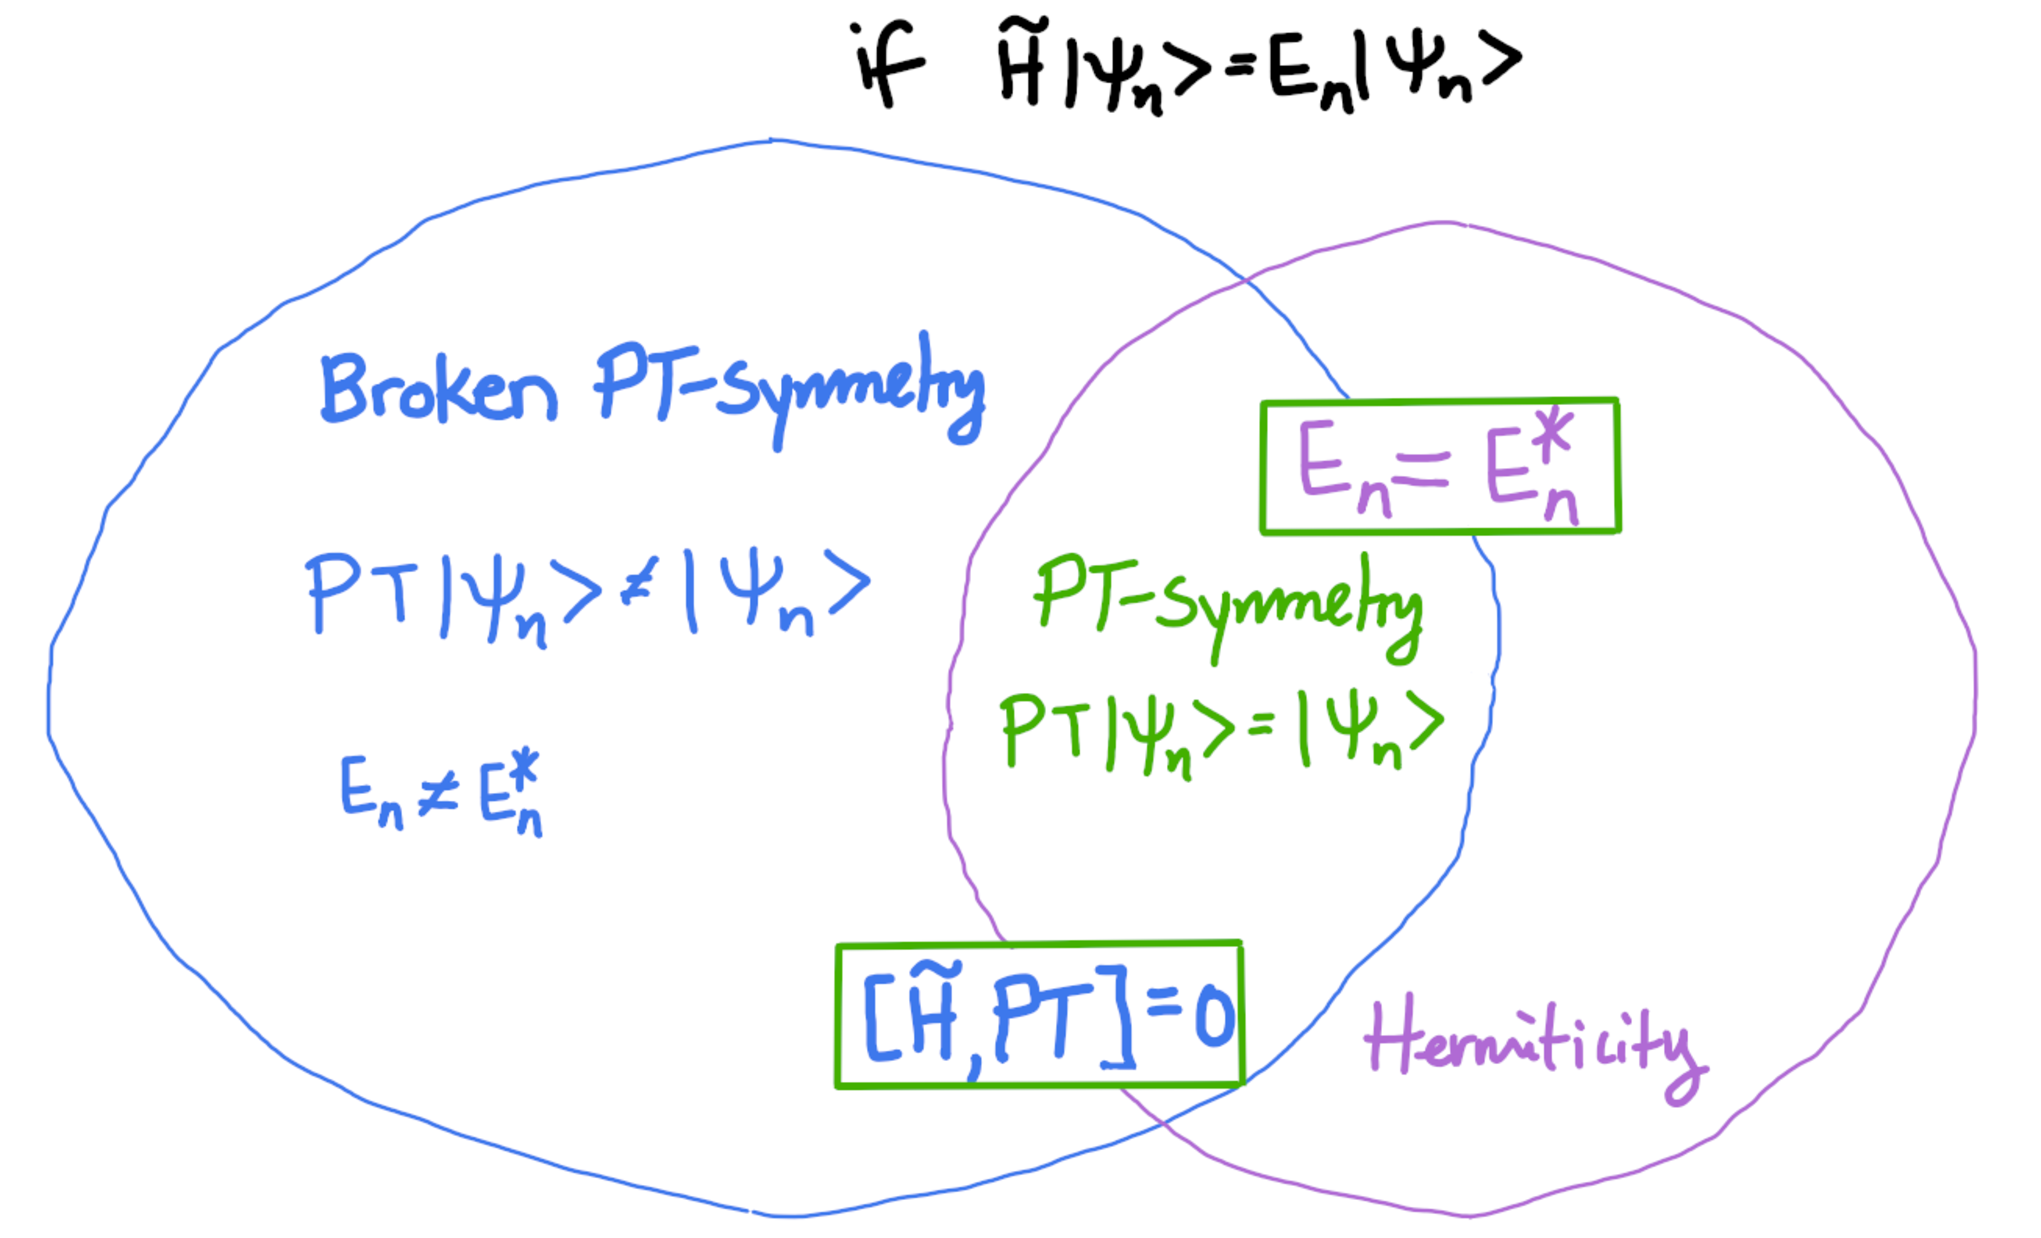
\includegraphics[width=0.6\linewidth]{eigenvalues_and_PTsymmetry.pdf}
\captionof{figure}{Reproduction of Fig.~2 in~\cite{Faria1}. This is an illustration of the conditions in equations \ref{eq:2.2}. The details in this figure are subtle. Unbroken or exact \PT-symmetry requires that both conditions in \ref{eq:2.2} are true. iSnce the \PT\:operator is antilinear it is possible that eigenstates of a Hamiltonian are not also eigenstates of the \PT operator depite having commutation between the  Hamiltonian and the \PT\: operator.}
\label{fig:eigenvalues}
\end{Figure}
Most model \PT-symmetric Hamiltonians $\tilde{H}$ in the literature admit tunable parameters such that there will be regions in the parameter space where the eigenstates of $\tilde{H}$ are not \PT-symmetric~\cite{Brody_2013}. This means that a system described by $\tilde{H}$ admits two phases, one for broken and another for unbroken \PT-symmetry. In the unbroken phase eigenstates of $\tilde{H}$ become degenerate and this implies that they lose completeness~\cite{Brody_2013}.
The effectiveness of \PT\:symmetry as a tool to investigate the spectra of some non-Hermitian Hamiltonians has been shown in various works, such as Dorey et al.~\cite{Dorey_2001, Dorey_2004}, Bender and Boettcher~\cite{RealSpectrainNHH}, Brody~\cite{Brody_2016}, Bender and Mannheim ~\cite{Bender_2010}, Bender et al.~\cite{PTsymmetricQM}, Weigert~\cite{Weigert_2003} among others.
To ensure that the eigenstates $\{\ket{\psi_n}\}$ of a \PT-symmetric Hamiltonian $\tilde{H}$ are orthogonal, it is necessary to specify an inner product. A possible choice for the inner product associated with $\tilde{H}$ might be~\cite{PTsymmetricQM}
\begin{equation}\label{eq:2.3}
\braket{\psi_n|\psi_m} \equiv \int_{c} dx [\psi_{n}(x)]^{\mathcal{PT}}\psi_m(x) = \int_{c} dx [\psi_{n}(-x)]^{*}\psi_m(x)
\end{equation}
where $c$ is a complex contour that starts and ends within specific boundary conditions (see Sec.~\ref{Stokes}). Unfortunately this obvious choice for the \PT\:inner product is not correct because it does not guarantee a positive definite norm~\cite{MakingSense}.

%%%%%%%%%%%%%%%%%%%%%%%%%%%%%%%%%%%%%%%%%%%%%%%%%%%%%%%%%%%%%%%%%%%%%%%%%%%%%%%%%%%%%%%%%%%%%%%
\section{The \texorpdfstring{$\mathcal{CPT}$}\:\:inner product}\label{CPT}
To be able to describe precisely the nature of \PT-symmetric quantum mechanics, we must delve briefly into the inner-product under which our theory satisfies the postulates of conventional quantum mechanics. It is important to note that \PT-symmetric quantum mechanics is a kind of `bootstrap' theory~\cite{MakingSense}, since infinitely many inner-products exist for a given vector space, we can construct an inner product whose associated norm is positive definite by design. This inner-product is in general dependent on the characteristics of the Hamiltonian in question and it guarantees that the underlying dynamics of any \PT-symmetric Hamiltonian satisfies unitarity~\cite{MustaHbeHermitian}.
Firstly, it is necessary to solve for the eigenstates of the Hamiltonian before knowing the Hilbert space and consequentially the associated inner product.
To guarantee a positive norm for our theory, we will construct a new linear operator \CC\:that commutes with both $\hat{H}$ and \PT. We use the symbol \CC\: to represent this symmetry because its properties are similar to those of the charge conjugation operator in particle physics~\cite{MakingSense}.

%%%%%%%%%%%%%%%%%%%%%%%%%%%%%%%%%%%%%%%%%%%%%%%%%%%%%%%%%%%%%%%%%%%%%%%%%%%%%%%%%%%%%%%%%%%%%%%
\subsection{The $\mathcal{C}$ operator}\label{CC}
When the \PT-symmetry of $\hat{H}$ is unbroken, the eigenfunctions $\psi_n(x)$ of $\hat{H}$ are simultaneously eigenstates of the \PT\:operator~\cite{Bender_2004}
\begin{equation}\label{eq:2.4}
\mathcal{PT}\psi_n(x) = \lambda_n \psi_n(x),
\end{equation}
Where $\lambda_n$ is a pure phase. Without loss of generality, for each $n$\:the phase can be absorbed into $\psi_n(x)$ and this makes the eigenvalue of the \PT operator unity~\cite{Bender_2004}: 
\begin{equation}\label{eq:2.5}
\mathcal{PT}\psi_n(x) = \psi_{n}^{*}(-x) = \psi_n(x).
\end{equation}

There is strong evidence of the completeness of the eigenfunctions $\psi_n(x)$~\cite{ComplexExtension, Bender_2004, Brody_2013}. In the coordinate basis, the completeness statement reads:
\begin{equation}\label{eq:2.6}
\sum_{n}(-1)^{n}\psi_n(x)\psi_n(y) = \delta(x-y),\quad x, y \in \mathbb{R}
\end{equation}
the unconventional $(-1)^n$ factor in \ref{eq:2.6} can be explained if we define the \PT\:inner product as the one in equation \ref{eq:2.3}. In contrast with a Hermitian Hamiltonian--which always commutes with a parity operator--the definition in \ref{eq:2.7} describes how eigenstate norms alternate in sign depending on the value $n$. 
This means that the metric associated with the \PT\: inner product is indefinite~\cite{Bender_2004,Critique}.
In quantum theory, the norm of states is interpreted as a probability and this means that the indefinite metric described above presents a serious problem for the validity of \PT-symmetric quantum theory. The solution to this problem lies in finding an interpretation for the negative valued norms~\cite{PTsymmetricQM}.

The literature claims that for any theory with unbroken \PT-symmetry there exists a symmetry of the Hamiltonian that describes the negative and positive norm states. To describe this symmetry of $\hat{H}$ it is necessary to construct a linear operator denoted by \CC~\cite{MustaHbeHermitian,ComplexExtension,Bender_2004}. When represented in position space \CC\: is a sum over the energy eigenstates of $\hat{H}$:
\begin{equation}\label{eq:2.7}
\mathcal{C} = \sum_n \psi_n(x)\psi_n(y)
\end{equation}
From this definition, relation $(\psi_m(y), \psi_n(y)) = \int dy\:(\mathcal{PT}\psi_m(y))\psi_n(y)$ and equation \ref{eq:2.5} we can verify that the eigenvalues of \CC\: are $\pm 1$
\begin{align}\label{eq:2.8}
\mathcal{C} \psi_n(x) & = \int dy\:\mathcal{C}\:\psi_n(y)\nonumber \\
& = \sum_{m}\psi_m(x)\int dy\:\psi_m(y) \psi_n(y)\nonumber \\
& = (-1)^n \psi_n(x)
\end{align}
The \PT\:norm signatures can therefore be interpreted as the ``charge'' of the states, while \CC\: is the operator used to measure this charge~\cite{Bender_2004}. The \CC\: operator commutes with the \PT\: operator, but it does not commute with the parity operator \PP. Notice that \CC\:and \PP\: operators are square roots of $\delta(x-y)$ the unity operator~\cite{ComplexExtension}
\begin{equation}\label{eq:2.9}
\mathcal{P}^2 = \mathcal{C}^2 = \mathds{1}, 
\end{equation}
where $\mathcal{P} \neq \mathcal{C}$, since \PP\: is real and \CC\: is complex valued~\cite{MustaHbeHermitian, Bender_2004}.

Using the newly constructed \CC\: operator, we can redesign the \PT\: inner product to suit the conventional probabilistic interpretation of the vector norms in quantum mechanics
\begin{equation}\label{eq:2.10}
\left( f, g \right ) = \int dx \left [ \mathcal{CPT} f(x) \right ] g(x).
\end{equation}
We must point out that all experimental evidence to date shows that nature follows the Dirac inner-product~\cite{Maximal}. However, the definitions given above show much promise as they might allow us to study non-Hermitian dynamics in experimental set-ups.

%%%%%%%%%%%%%%%%%%%%%%%%%%%%%%%%%%%%%%%%%%%%%%%%%%%%%%%%%%%%%%%%%%%%%%%%%%%%%%%%%%%%%%%%%%%%%%%%%%%%%%%%%%%
\section{$2\times2$ \PT-symmetric Hamiltonian}\label{2x2}
An example of the results of unbroken \PT-symmetric theory that is often found in the literature describes a simple finite non-Hermitian but \PT-symmetric Hamiltonian
\begin{equation}\label{eq:2.11}
\tilde{H} = \begin{pmatrix}
re^{i\theta} & s  \\
s & re^{-i\theta} \\
\end{pmatrix},
\end{equation}
where the parameters $r, s$ and $\theta$ are real. In this set-up the \TT\: operator performs complex conjugation and the parity operator is written as
\begin{equation}\label{eq:2.12}
\mathcal{P} = \begin{pmatrix}
0 & 1  \\
1 & 0 \\
\end{pmatrix}.
\end{equation}

We can show that the Hamiltonian in \ref{eq:2.11} is \PT-symmetric
\begin{equation*}
\mathcal{PT}\tilde{H}\mathcal{PT} =\begin{pmatrix}
0 & 1  \\
1 & 0 \\
\end{pmatrix}
\begin{pmatrix}
re^{-i\theta} & s  \\
s & re^{i\theta} \\
\end{pmatrix}
\begin{pmatrix}
0 & 1  \\
1 & 0 \\
\end{pmatrix} = \tilde{H}.
\end{equation*}
The \ref{eq:2.11} Hamiltonian is written in operator form as $\tilde{H} = r\cos\theta \hat{\mathbb{I}} + \frac{\omega}{2} \vec{\sigma}\cdot\hat{n}$, where $\vec{\sigma}$ is the three dimensional Pauli vector and $\hat{n}$ is a normal vector. The eigenvalues of this Hamiltonian are $E_{\pm} = r\cos\theta \pm \sqrt{s^2 - r^2\sin^2\theta}$. We can see that the Hamiltonian allows two parametric regions. When $s^2 < r^2\sin^2\theta$ the eigenvalues of $\tilde{H}$ form a complex conjugate pair. This is the broken \PT-symmetry region. Otherwise, when $s^2 \geq r^2\sin^2\theta$, then the eigenvalues are real. This is the region of unbroken \PT-symmetry region. In the unbroken symmetry region the \PT\:normalised eigenstates of both $\tilde{H}$ and \PT\:are
\begin{equation}\label{eq:2.13}
\ket{E_{+}} = \frac{1}{\sqrt{2\cos\alpha}}\begin{pmatrix}
e^{i\alpha/2} \\
e^{-i\alpha/2} \\
\end{pmatrix}\quad\mathrm{and}\quad\ket{E_{-}} = \frac{i}{\sqrt{2\cos\alpha}}\begin{pmatrix}
e^{-i\alpha/2} \\
-e^{i\alpha/2} \\
\end{pmatrix},
\end{equation}
we use the relation $\sin\alpha = \frac{r}{s}\sin\theta$. The corresponding \CC\:operator for this Hamiltonian is 
\begin{equation}\label{eq:2.14}
\mathcal{C} = \frac{1}{\cos\alpha}\begin{pmatrix}
i\sin\alpha & 1 \\
1 & -i\sin\alpha\\
\end{pmatrix}.
\end{equation}
This \CC\:operator commutes with $\tilde{H}$ and satisfies $\mathcal{C}^2= \mathds{1}$. The eigenvalues of \CC\:are precisely the signs of the \PT\:norms of the corresponding eigenstates~\cite{Bender_2004}. Using this \CC\: operator we can guarantee that the \CC\PT\:inner product in the two-dimensional Hilbert space spanned by $\ket{E_{\pm}}$ is positive definite.

%%%%%%%%%%%%%%%%%%%%%%%%%%%%%%%%%%%%%%%%%%%%%%%%%%%%%%%%%%%%%%%%%%%%%%%%%%%%%%%%%%%%%%%%%%%%%%%
\chapter{Broken \PT-symmetry}\label{EPs}
In contrast with unbroken symmetry, Hamiltonians with broken \PT-symmetry do not satisfy the spectral theorem and this gives rise to very unconventional quantum mechanical behaviour. Hamiltonians with broken \PT-symmetry exhibit purely non-Hermitian spectral degeneracies known as exceptional points (EP)~\cite{Bossart}.
EPs are points in an (at least) two-dimensional parameter space, in which two or more eigenstates "coalesce" and become identical~\cite{Moiseyev, Cartarius}. That is, in the presence of EPs, the coalescence of eigenstates causes the collapse of the subspace dimension to one, because of this the eigenstate no longer forms a complete basis~\cite{Bagarello}. The interest in these degeneracies has increased greatly since they give rise to dramatic effects in a great variety of physical problems: in mechanics, electromagnetism, atomic and molecular physics, quantum phase transitions, quantum chaos and more~\cite{Heiss_2012}.
An illustrative example of EPs can be seen when we consider the well known family of \PT-symmetric Hamiltonians
\begin{equation}\label{eq:3.1}
\hat{H} = \hat{p}^2 + \hat{x}^{2}(i x)^{\epsilon} \quad\quad (\epsilon\:\mathrm{real}). 
\end{equation}
These Hamiltonians have unbroken \PT\:symmetry when $\epsilon \geq 0$ and broken \PT-symmetry when $\epsilon < 0$~\cite{MakingSense}. The energy spectrum of \ref{eq:3.1} has been proved to be real and bounded below in the region of unbroken \PT\:symmetry ~\cite{Dorey_2004}. In Fig.~\ref{fig:parametricfam} I present my numerical results demonstrating both these symmetry regions and the visible \PT\:phase transition that characterizes the spectra of these parametric Hamiltonians.
\begin{Figure}
\centering
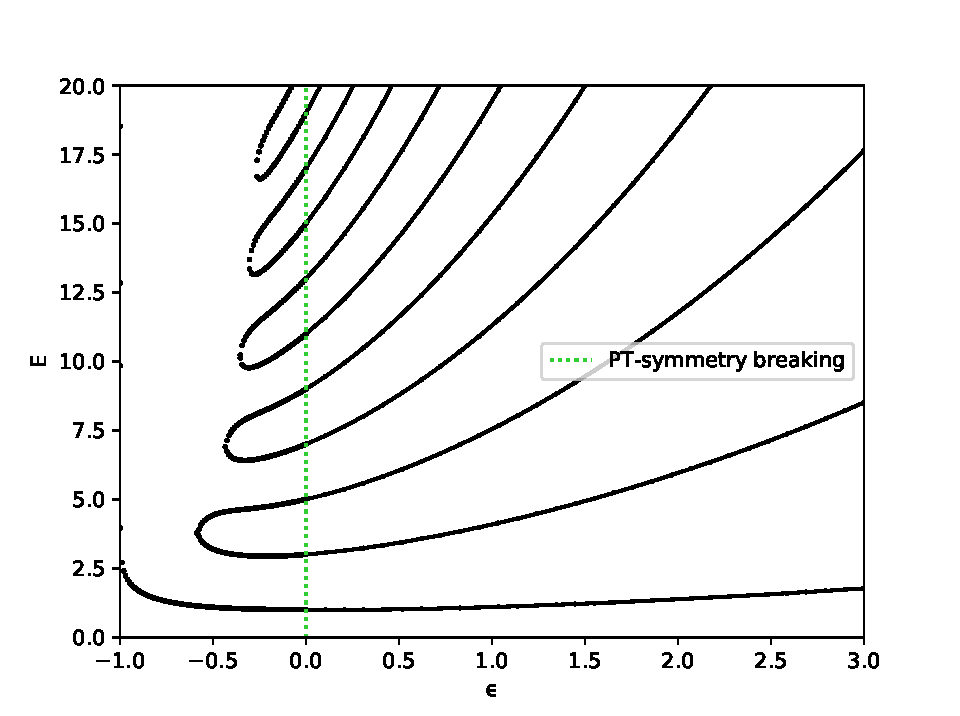
\includegraphics[width=0.6\linewidth]{parametric_fam.pdf}
\captionof{figure}{Reproduced from Fig.~1 in~\cite{MakingSense}. This plot exemplifies the behaviour of the eigenvalue spectra of the Hamiltonians in \ref{eq:3.1} as a function of the real parameter $\epsilon$. All the eigenvalues visible in this figure are real valued. The vertical dotted green line corresponds to the value $\epsilon = 0$, this is the point where \PT-symmetry breaks and it corresponds to the Hamiltonian for the classic one dimensional harmonic oscillator. When $\epsilon \geq 0$ the spectra are real, positive and discrete. Energy levels increase with increasing $\epsilon$. In the region corresponding to $-1 \leq \epsilon \leq 0$ there is a finite number of real positive eigenvalues and an infinite number of complex-conjugate pairs of eigenvalues (not depicted). The number of real eigenvalues decreases as $\epsilon$ decreases from $0$ to $-1$, for $\epsilon$ that are more negative than the value $\epsilon = -0.57793$ the only remaining real eigenvalue corresponds to the ground-state energy. At the value $\epsilon = -1$ the spectrum is null  as all eigenvalues diverge towards positive infinity.}
\label{fig:parametricfam}
\end{Figure}
In Ch.~\ref{MINE} we will investigate the unbroken symmetry region of Fig.~\ref{fig:parametricfam}, specifically the case for $\epsilon = 2$. However since in this section we are concerned with EPs, we must zoom into the parametric region $\epsilon < 0$. The broken \PT-symmetry region is visible in more detail in Fig.~\ref{fig:broken_region}.
\begin{Figure}
\centering
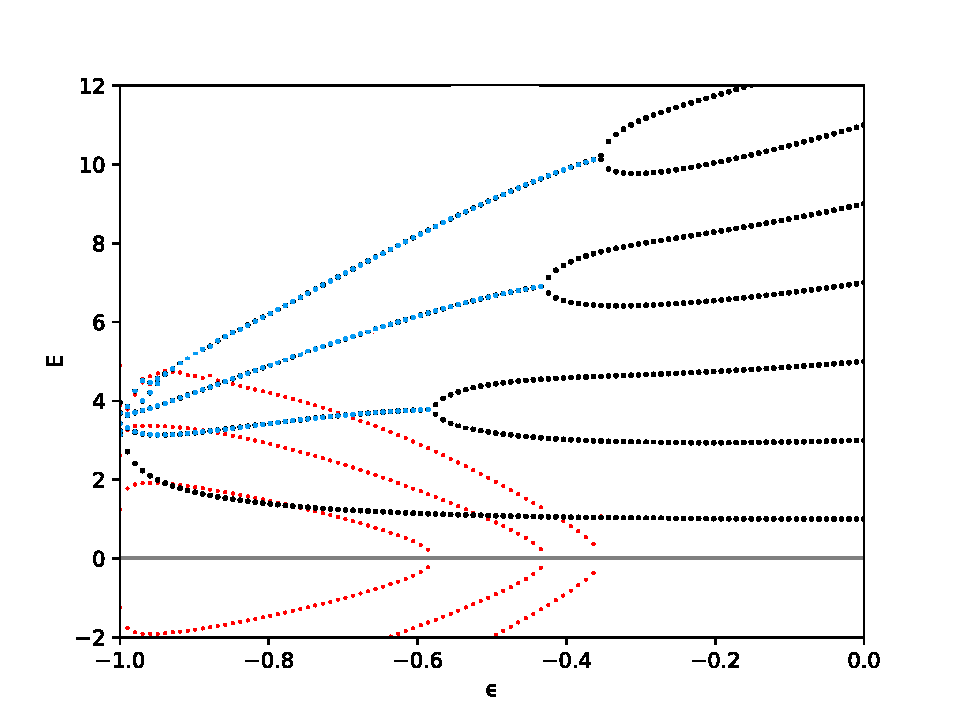
\includegraphics[width=0.6\linewidth]{broken_region.pdf}
\captionof{figure}{Reproduced from Fig.~3 in~\cite{BrokenRegion}. Similarly to Fig.~\ref{fig:parametricfam}, this is the eigenvalue spectra of the Hamiltonians in \ref{eq:3.1} as a function of the real parameter $\epsilon$ in the case where $\epsilon < 0$. A parameter space for $\epsilon$ is depicted as 100 values in the horizontal axis, and the energy range $-2 \leq E \leq 12$ as the vertical axis. Fully real eigenvalues are presented as black dots. Visible here are three epsilon values at which the real eigenvalues become degenerate (coalesce) and then form complex-conjugate pairs. The real parts of these pairs of eigenvalues are represented as blue dots. These energies initially decrease as $\epsilon$ decreases but diverge suddenly as $\epsilon$ approaches $-1$ (The divergence of the real-parts was not captured by my numerics). The imaginary parts of the eigenvalue pairs are represented as red dots. These remain finite and appear to decay to zero at $\epsilon = -1$.}
\label{fig:broken_region}
\end{Figure}
In Fig.~\ref{fig:broken_region} there are three visible EPs of order 1 and a single infinite order EP at $\epsilon=-1$. 
It is numerically difficult to resolve the infinite order EP, as can be seen by the noisy data as we approach $\epsilon=-1$

As shown in both Figs.\ref{fig:parametricfam} and \ref{fig:broken_region} EPs degeneracies can be points where eigenvalues and the wave functions are interchanged, For example, if the EP corresponds to a cubic root branch point. For a closed contour around this point a cyclic permutation of all three eigenvalues and eigenfunctions is then expected~\cite{Cartarius}. This effect has an important consequence on time evolution. Time evolution at EPs differs from generic Hamiltonians in the sense that only one state evolves with the usual oscillations (possibly with overall damping or amplification), while other states remain inextricably coupled to this single eigenstate~\cite{Bossart}. 

%%%%%%%%%%%%%%%%%%%%%%%%%%%%%%%%%%%%%%%%%%%%%%%%%%%%%%%%%%%%%%%%%%%%%%%%%%%%%%%%%%%%%%%%%%%%%%%
\chapter{Time evolution}\label{TEv}
In Hermitian quantum mechanics, time-evolution of states is done by using the unitary operator $\hat{U} = e^{-i\hat{H}t/\hbar}$. Because the $\hat{U}$ operator is unitary this means that as the state $\vec{\psi}$ evolves in time, its norm remains constant. This is useful in quantum mechanics because the norm of a state is interpreted as a probability, and therefore unitarity guarantees that a state's probability does not grow or decay with time. As explained in Sec.\ref{CPT}, when the \PT-symmetry of $\hat{H}$ is unbroken it is possible to have positive definite \CPT norm states for the non-Hermitian Hamiltonian. This means that time evolution under the unbroken \PT-symmetric framework is also unitary~\cite{Jones-Smith, ComplexExtension, Mostafazadeh2}. 
The unitary time evolution of a state $\vec{\psi}$ from time $t = 0$ to a time $t$ is written as
\begin{equation}\label{eq:4.1}
\vec{\psi}(t) = \hat{U} \vec{\psi}(0).
\end{equation}
An interesting feature of \PT-symmetric Hamiltonians has been suggested in ~\cite{Bender_2007}. According to this paper it is possible to obtain arbitrarily fast quantum evolutions using non-Hermitian \PT-symmetric Hamiltonian operators. This is because for such Hamiltonians the path from can be made short by taking advantage of the Hilbert space geometry described by the Hamiltonian's eigenstates. A brief description of this work is described below.
%>>>MOREEEEEEEE ON GEOMETRYYYYYA brief description of this work is described below.

%%%%%%%%%%%%%%%%%%%%%%%%%%%%%%%%%%%%%%%%%%%%%%%%%%%%%%%%%%%%%%%%%%%%%%%%%%%%%%%%%%%%%%%%%%%%%%%
\section{Faster than Hermitian time evolution?}\label{faster}
The mechanism described in Ref.~\cite{Bender_2007} is similar to that in general relativity in which the distance between two space-time points can be made small if they are connected by a wormhole. If true, the results in ~\cite{Bender_2007} will have drastic consequences in quantum computation, because it removes the bound on time-optimal unitary operations~\cite{OptimalControl} that is established in quantum mechanics~\cite{Brachistochrone_Mostafazadeh}. However, Bender et al. warn us about the possibility of the existence of quantum protection mechanisms that place a lower bound on the time required to switch Hilbert spaces, which would limit the applicability of a Hilbert-space ``wormhole" to improve quantum algorithms~\cite{Bender_2007}. 

G\"{u}nther and Samsonov~\cite{Gunther_2008} have interpreted the \PT-symmetric set-up for Ref.~\cite{Bender_2007} as a quantum system consisting of a non-Hermitian \PT-symmetric component and a Hermitian component simultaneously. G\"{u}nther and Samsonov formulate a general recipe for the construction of partially \PT-symmetric quantum
systems which are not 1:1 equivalent to purely Hermitian systems. Using a strong structural analogy with the
reference frames for inertial observers in special relativity, they associate \PT-symmetric models in different
representations with corresponding measurement frames. They claim that the resultant operators which are Dirac Hermitian
are connected with non-Dirac-Hermitian operators in another frame. The probabilistic content of the models
is frame-independent. According to G\"{u}nther and Samsonov their geometric analysis of the equivalence mapping between mutually \PT-symmetric and Hermitian operators demonstrates the agreement of the vanishing passage-time solution proposed in ~\cite{Bender_2007} and the temporal lower bound for Hermitian evolution proposed by Anandan and Aharonov in ~\cite{AnandanAharonov}. 

Despite the potential importance of \PT-symmetric theory, the experimental observation in a genuine quantum system is still missing~\cite{Cartarius}. Therefore the purpose of our research is to determine whether it is possible to observe the dynamical behaviour of a \PT-symmetric quantum in an experiment. 

%%%%%%%%%%%%%%%%%%%%%%%%%%%%%%%%%%%%%%%%%%%%%%%%%%%%%%%%%%%%%%%%%%%%%%%%%%%%%%%%%%%%%%%%%%%%%%%
\chapter{Experiments}\label{Experiments}
Much research has been carried out on properties of physical systems described by \PT-symmetry. Such Hamiltonians can be used to model the behaviour of closed quantum systems, but they can also be replicated in open systems which exhibit balanced gain and loss. This has been implemented in laboratory experiments for a wide range of systems~\cite{geometric_aspects}, here are some brief examples.

\section{Observation of a Topological Transition in the Bulk of a Non-Hermitian System}\label{TopologicalTrans}
The work of Zeuner et al. in ~\cite{TopoTrans} describes topological transitions in a non-Hermitian system. 
Topological transport is a chiral transport phenomenon of particles due to Hall conductance that can be linked to an integer-valued topological quantity. This kind of phenomenon has been observed in two-dimensional electron gases, silicon platforms, and even in ultra-cold gases~\cite{TopoTrans}. 

Zeuner et al. present an experiment where they realise the idealised one-dimensional non-Hermitian dimer model. The model used in this investigation permits the loss or absorption of transported particles at every second site of a one-dimensional optical lattice. It is this phenomenological loss of particles that makes the system non-Hermitian. The experimental methodology is based on bulk measurements of topological transitions in fabricated waveguide lattices with alternating distances in fused silica glass.
To introduce loss, every second waveguide is sinusoidally oscillated transversely to the plane of the waveguides~\cite{TopoTrans}.
The results of this experiment leads Zeuner et al. to argue that the features of the idealized tight binding model in~\cite{Rudner} carries over to experiments. Because loss is an inherent feature of many systems that may exhibit topological effects (such as coupled quantum dots~\cite{Rudner}, and driven-dissipative exciton-polariton condensates ~\cite{Cones}). This intrinsic non-Hermiticity may act as a surprising probe of their potentially rich topological phases~\cite{TopoTrans}.

\section{Light Stops at Exceptional Points}\label{StopLight}
In 2018 Goldzak et al. published ~\cite{LightStopsatEPs} where they relate stationary light pulses and the phenomenon of an exceptional point (EP). In their work they claim to conceptually show that the group velocity of light vanishes if a waveguide is designed exactly at the EP. Goldzak et al. explain that this pulse-stop effect is possible in a PT-symmetric optical waveguides where two optical modes coalesce. \PT-symmetry is characterized by accurately balanced loss and gain in time. 

In their proposed experiment Goldzak et al. ``freeze'' and release Gaussian light pulses by adiabatically increasing gain and loss parameters. Using a pumped optical cavity as the non-linear medium, Goldzak et al. explain that parametric interactions operating at ultra fast rates can be engineered using synchronously pumped optical parametric oscillators ~\cite{LightStopsatEPs}. After the light pulse is ``released'' it should be possible to observe that the carried coherent information is preserved. They explain that it is the non-resonant mechanism of this phenomenon that is of an important technological advantage, since apparently this result can be tuned for optical pulses in a wide range of frequencies and bandwidths. In addition they propose that it should be possible to engineer this effect in any \PT-symmetric system of two waveguide channels. which in theory should not be limited only to light but could be extended to acoustic waves or other fields in physics satisfying \PT-symmetry~\cite{LightStopsatEPs}.
If replicable this result would open new possibilities for designing slow light devices, which would
exploit generic properties of EPs offering interesting operational capabilities of a new generation of photonic devices~\cite{LightStopsatEPs}.

\section{Topological protection in non-Hermitian Haldane honeycomb lattices}\label{TopoProtecc}
The work by Res\'endiz-V\'azquez et al. focuses in the possibility of observing topologically protected
edge states in two-dimensional non-Hermitian Haldane lattices~\cite{Tprotecc}.
The Haldane model represents a unique system where the quantum Hall effect is contained as an intrinsic lattice-band-structure property, rather than an external effect due to the presence of a strong magnetic
field~\cite{QuantumAnomalousEffect}. 

The claim in this paper is that edge states can be observed in the so-called broken PT -symmetric phase. 
The experiment is done using finite rectangular Haldane ribbon comprising 1860 sites. They present
the results for a lattice several kinds of terminations. Res\'endiz-V\'azquez et al. find that such topologically protected edge states emerge irrespective of the lattice boundaries, namely, zigzag, bearded, or armchair.which implies that, in general, the edge geometry of the sample does not play a role in the observation of topological edge protection as long as the system is described by a ribbon. This contrasts with previous findings. The results reported by Res\'endiz-V\'azquez et al. help elucidate the role of
\PT-symmetry in two-dimensional topological phenomena and demonstrate that topological protection can exist in the archetypal Haldane model even in the presence of gain and loss~\cite{Tprotecc}.\\

There is an ongoing quest devoted to investigating the advantages of extending quantum theory via \PT-symmetry. On occasion this has revealed new phenomena apparently exclusive to non-Hermitian systems, to read more on this please refer to ~\cite{EigenspaceEPs} and ~\cite{NHQuantumHall}.

%%%%%%%%%%%%%%%%%%%%%%%%%%%%%%%%%%%%%%%%%%%%%%%%%%%%%%%%%%%%%%%%%%%%%%%%%%%%%%%%%%%%%%%%%%%%%%%
\chapter{Project statement}\label{MINE}
We are interested in understanding the dynamics of quantum mechanical super fluids in non-Hermitian traps. Our ultimate goal in this project is to fully develop a \PT-symmetric model describing the evolution of a Bose-Einstein condensate after a quench transforms an initial three-dimensional Hermitian potential into a non-Hermitian \PT-symmetric trap in the shape of an inverted quartic in one dimension. We would also potentially extend this model to three-dimensions. 

In Sec.~\ref{EPs} we described the parametric family of \PT-symmetric Hamiltonians in \ref{eq:3.1}. As explained previously, these Hamiltonians have unbroken \PT\:symmetry when $\epsilon \geq 0$ and broken \PT-symmetry when $\epsilon < 0$. The particular Hamiltonian that we use in my project occurs when we let $\epsilon = 2$ in \ref{eq:3.1}. Our Hamiltonian is 
\begin{equation}\label{eq:6.1}
\tilde{H} = \hat{p}^2 - \hat{x}^{4},
\end{equation}
this Hamiltonian is interesting because even though it possesses an upside-down potential, it nevertheless appears to have a fully real and bounded below energy spectrum~\cite{UpsideDownPotentials} as can be seen in Fig.~\ref{fig:parametricfam}. 

The boundary conditions imposed on the eigenstates of \ref{eq:6.1} are
\begin{align}\label{eq:6.2}
\lim_{|x|\rightarrow \infty} \psi_n(x) &= 0, \nonumber\\
\mathrm{if}-\frac{\pi}{3} < \mathrm{arg}(x) < 0 \quad\mathrm{and}\quad&-\pi < \mathrm{arg}(x) < -\frac{2\pi}{3},
\end{align}
notice that these boundary conditions exclude the real-x axis. Solving the Schr\"{o}dinger equation for \ref{eq:6.1} requires integration along a contour whose ends lie in these wedges in the complex-x plane~\cite{UpsideDownPotentials} (see Fig.~\ref{fig:contour}).
\begin{Figure}
\centering
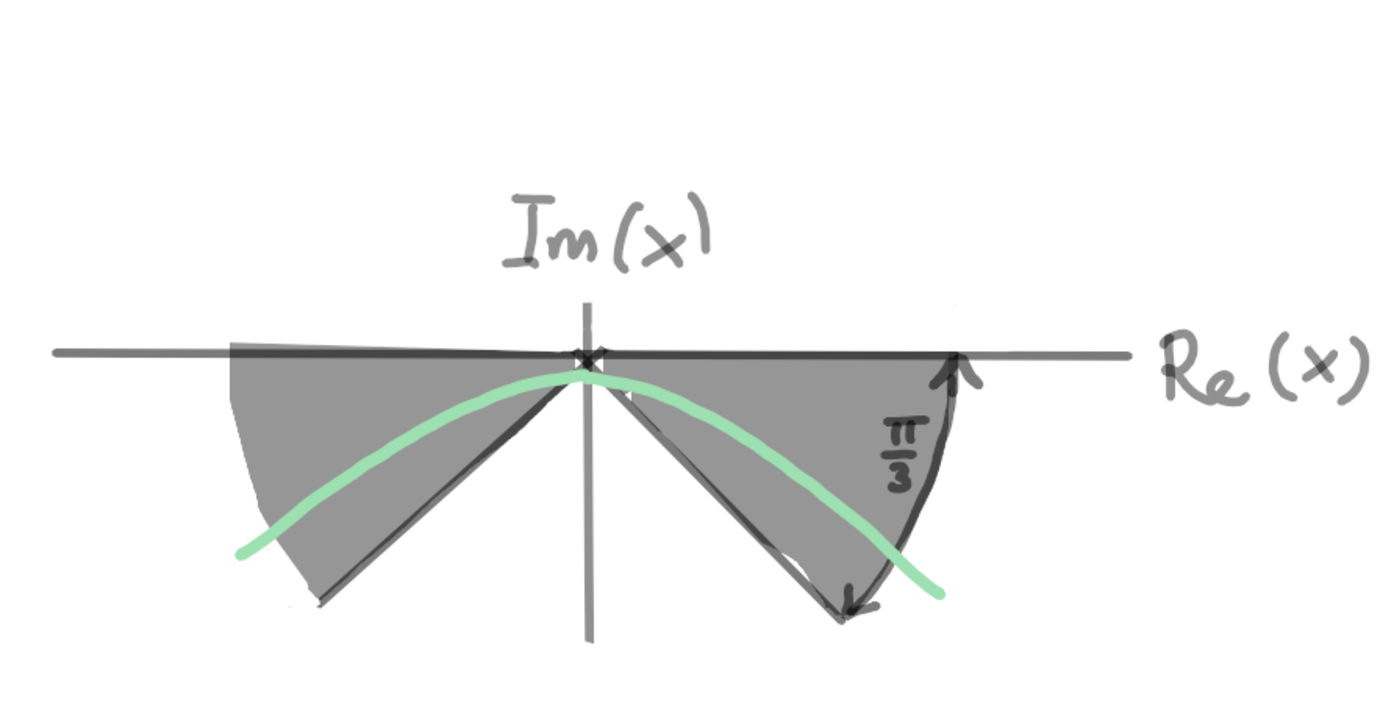
\includegraphics[width=.6\linewidth]{contour.pdf}
\captionof{figure}{Example of a possible complex contour used to solve the Schr\"{o}dinger equation for \ref{eq:6.1}. The contour is located within the pair of Stokes' wedges suitable for this Hamiltonian. The wedges lie in the lower half of the complex x-plane. Inside these wedges, the eigenfunctions of \ref{eq:6.1} decay exponentially as $|x| \rightarrow \infty$. Reproduced from ~\cite{UpsideDownPotentials}.}
\label{fig:contour}
\end{Figure}

For more details on boundary conditions and integration contours in the complex plane see appendix \ref{Stokes}.

%%%%%%%%%%%%%%%%%%%%%%%%%%%%%%%%%%%%%%%%%%%%%%%%%%%%%%%%%%%%%%%%%%%%%%%%%%%%%%%%%%%%%%%%%%%%%%%
\section{Simulation:\\ Time evolution of a quantum state}\label{nonPTsim}
Initially, my simulations were not fully informed by the \PT-symmetric framework, since originally I did not understand the importance of the \CPT\:inner product.
One of my simulations relied in the fourth-order Runge-Kutta algorithm (RK4). A few frames from my RK4 simulation are included in Fig.~\ref{fig:RK4}, where an interesting re-focusing effect appears to occur. Originally we were unsure if this effect was actually occurring physically of whether it was an artefact of the numerics.
\begin{Figure}
\centering
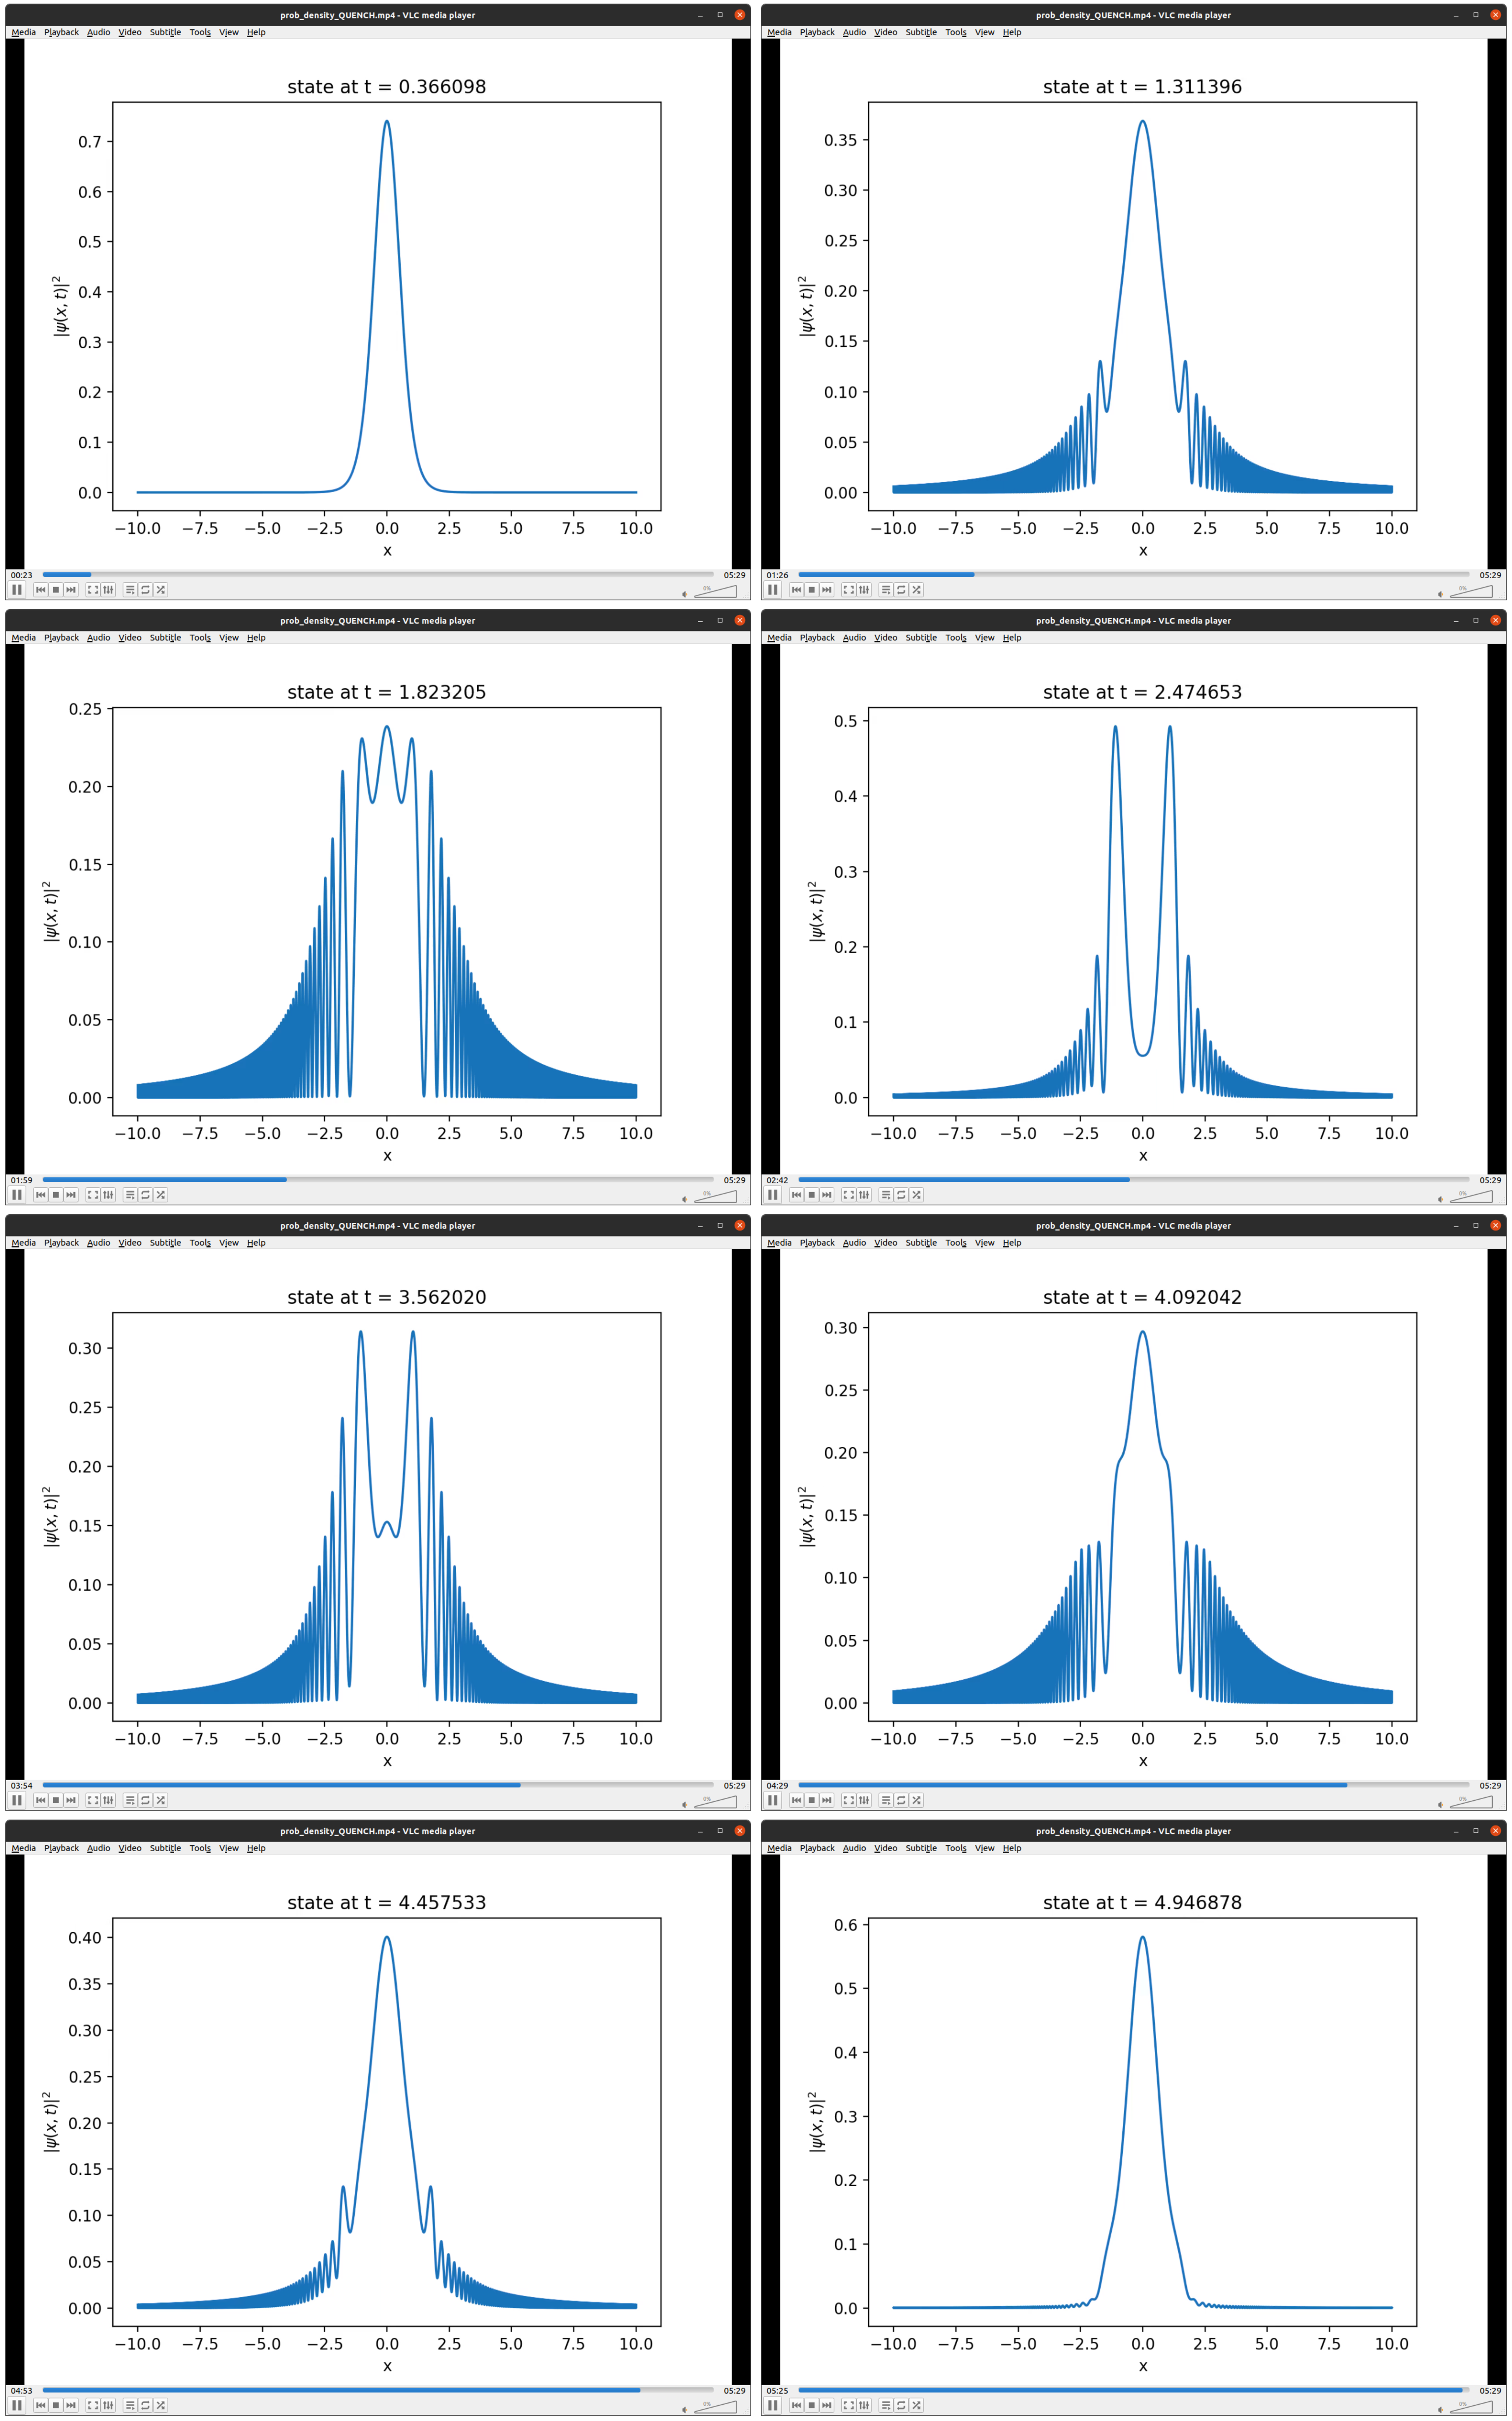
\includegraphics[width=.7\linewidth]{probability_density_in_negquartic.pdf}
\captionof{figure}{Eight frames in a time evolution simulation written using RK4. This figure should be read from top left to bottom right. This simulation implements time evolution by repeatedly solving the Schr\"{o}dinger equation for the Hamiltonian in \ref{eq:6.1} using the iterative RK4 algorithm. From the earliest frame (top left) to the latest frame (bottom right) a refocusing of the state can be seen as the state is allowed to evolve in the negative quartic potential trap.}
\label{fig:RK4}
\end{Figure}
After reading the literature described in detail in Sec.~\ref{EqHH} we were interested in understanding the behaviour of states trapped in the Hermitian Hamiltonian with an equivalent energy spectrum to the non-Hermitian Hamiltonian in \ref{eq:6.1}~\cite{HHEquivalent, Equivalent_withanomaly, ParityAnomaly}. 
\begin{equation}\label{eq:6.3}
\hat{H} = \frac{\hat{p}^2}{2m} + 4g\hat{x}^4 - \sqrt{2g}\hat{x},
\end{equation}
\begin{Figure}
\centering
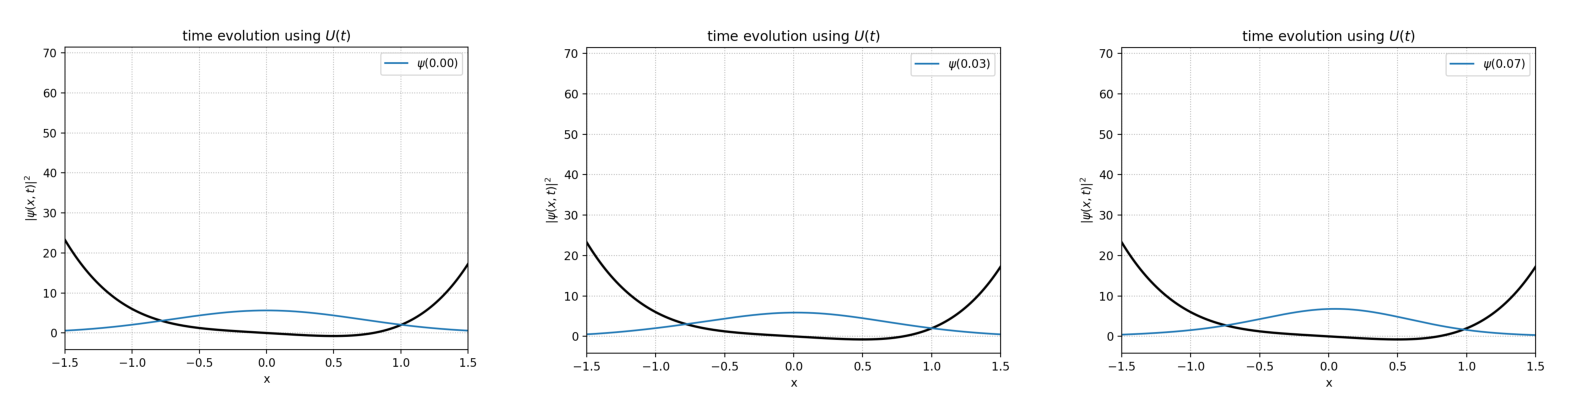
\includegraphics[width=\linewidth]{EHH_sim.pdf}
\captionof{figure}{Three frames from a time evolution simulation written using a unitary operator made using the Hermitian Hamiltonian  in \ref{eq:6.3}. The state trapped in this potential simply shifts back an forth along the x-axis but no other phenomena are observed as time passes.}
\label{fig:EHH_sim}
\end{Figure}
The simulations in both Fig.~\ref{fig:EHH_sim} and \ref{fig:RK4} gave us some insight about how certain pairs of non-Hermitian Hamiltonians and Hermitian Hamiltonians with equivalent energy spectra does not guarantee that the time evolution of states under these Hamiltonians will be equivalent or even similar.

\section{Simulation:\\ \PT-symmetric time evolution of a quantum state}
At this stage of my project I am using \PT-symmetry directly to implement the time evolution in my simulation. As described in in Ch.~\ref{TEv}, a Hamiltonian with unbroken \PT-symmetry can be used to make a unitary time evolution operator $\hat{U}$. In order to write the Hamiltonian matrix that will be required to make $\hat{U}$, I use the WKB approximation (outlined in Sec.~\ref{WKB}) to obtain an approximate numerical basis. These WKB basis wave functions are then \PT\:normalised and a \CC\:operator is constructed for the Hamiltonian in equation~\ref{eq:6.1}. The inner product used to generate the Hamiltonian matrix elements is none other than the \CC\PT\:inner product. This simulation is still a work in progress. 



%%%%%%%%%%%%%%%%%%%%%%%%%%%%%%%%%%%%%%%%%%%%%%%%%%%%%%%%%%%%%%%%%%%%%%%%%%%%%%%%%%%%%%%%%%%%%%%
\chapter{Conclusion}\label{Conclusion}
% Example overview and relevance
Although the Hermiticity postulate of quantum mechanics serves the theory well, not all non-Hermitian Hamiltonians describe physically invalid systems. Often, systems in nature interact with an environment and these interactions describe crucial features of said systems. A theory of non-Hermitian quantum mechanics can be used to investigate gain and loss interactions between a system and its surrounding environment. Non-Hermitian quantum mechanics can include an alternative to Hermiticity known as \PT-symmetry. This postulate has been shown to be consistent with all other aspects of the conventional quantum theory, which makes \PT-symmetric quantum theory a promising extension to conventional quantum mechanics. This review presents an introduction to \PT-symmetric quantum theory. This work delves briefly into the interesting phenomena of broken \PT-symmetry, including some examples of theoretical and experimental explanations for the unintuitive behaviour of eigenfunctions and eigenvalues in the presence of non-Hermitian degeneracies. Lastly, I present here the current stage of my investigations of \PT-symmetric quantum theory and its possible application to dynamical models of superfluids in non-Hermitian contexts.

% \section*{Acknowledgements}

%%%%%%%%%%%%%%%%%%%%%%%%%%%%%%%%%%%%%%%%%%%%%%%%%%%%%%%%%%%%%%%%%%%%%%%%%%%%%%%%%%%%%%%%%%%%%%%
\chapter{Appendix}\label{appendix}
\section{Bi-orthogonality and completeness}\label{Biorthogonal}
In the case of a \PT-symmetric Hamiltonian $\tilde{H}$, it is possible for two (or more) complex eigenvalues to cross. At the crossing point the eigenvalues are degenerate and this is accompanied by the coalescence of the eigenstates of $\tilde{H}$. If eigenstates of $\tilde{H}$ become degenerate this implies that they lose completeness~\cite{Brody_2013}. This special situation is associated with a branch point in the complex energy plane and is commonly termed an ``exceptional point"~\cite{Moiseyev}. Moreover, sufficiently close to the branch point the eigenfunctions of the coalescing eigenvalues are nearly self-orthogonal.

We need completeness and closure relations in order to develop, for example, perturbation theory and scattering theories for non-Hermitian Hamiltonians and in order to be able to solve the Schrödinger equation by numerical methods~\cite{Moiseyev}.

Suppose that a diagonalizable non-Hermitian Hamiltonian $\tilde{H}$ has a discrete spectrum and it commutes with the \PT\:operator. This means that  $\tilde{H}$ has unbroken \PT-symmetry. A Hilbert space $\mathcal{H}$ spanned by the eigenvectors of $\tilde{H}$ exists, but because $\tilde{H}$ is non-Hermitian --with respect to the standard inner product of $\mathcal{H}$-- the time evolution generated by $\tilde{H}$ will not be unitary~\cite{Mostafazadeh}. Nevertheless, as explained in section \ref{CC}. For the assumed $\tilde{H}$ above it is possible to construct a different complete positive-definite inner product by constructing and using the antisymmetric \CC\:operator that corresponds to $\tilde{H}$.

The assumed diagonalizability condition of $\tilde{H}$ may be viewed as a physical requirement without which an energy eigenbasis would not exist. To our knowledge all known non-Hermitian Hamiltonians that are used in physical applications are diagonalizable and therefore admit a complete \emph{bi-orthonormal} set of eigenvectors. This set of bi-orthonormal eigenvectors is $\{(\ket{\psi_{n}, a}, \ket{\phi_{n}, a})\}$ and will satisfy the following defining relations~\cite{Pseudo-HermiticityIII}
\begin{align}
\tilde{H}\ket{\psi_{n}, a} = E_{n}\ket{\psi_{n}, a},\quad\tilde{H^{\dagger}}\ket{\phi_{n}, a} &= E^{*}_{n}\ket{\phi_{n}, a},\\
\nonumber\\
\braket{\phi_{m}, b|\psi_{n}, a} = \delta_{mn}\delta_{ab}&,\\
\nonumber\\
\sum^{}_{n}\sum_{a=1}^{d_n}\ket{\psi_{n}, a}\bra{\phi_{n}, a} = \hat{\mathbb{I}}&\\
\tilde{H} = \sum^{}_{n}\sum_{a=1}^{d_n}E_{n}\ket{\psi_{n}, a}\bra{\phi_{n}, a},\quad\tilde{H^{\dagger}} &= \sum^{}_{n}\sum_{a=1}^{d_n}E_{n}^{*}\ket{\phi_{n}, a}\bra{\psi_{n}, a}
\end{align}
where $n$ and $a$ are the spectral degeneracy levels, $d_n$ is the degree of degeneracy of $E_n$ and $\hat{\mathbb{I}}$ is the identity operator~\cite{Pseudo-HermiticityIII}.

%%%%%%%%%%%%%%%%%%%%%%%%%%%%%%%%%%%%%%%%%%%%%%%%%%%%%%%%%%%%%%%%%%%%%%%%%%%%%%%%%%%%%%%%%%%%%%%
\section{Equivalent Hamiltonians with distinct symmetries}\label{EqHH}
In parallel to the work of Bender is the research of Mostafazadeh who introduced the notion of pseudo-Hermiticity in ~\cite{Mostafazadeh, Pseudo-HermiticityII, Pseudo-HermiticityIII, Mostafazadeh2, Mostafazadeh_2002}. Mostafazadeh has published works discussing his scepticism of the application of \PT-symmetry to quantum mechanics such as in~\cite{Critique}. He argues that importance of the Hermitian representation of the \PT-symmetric (and other) unitary quantum systems cannot be undermined by a demonstration that certain calculations take a simpler form in the non-Hermitian representation of these systems. Since there are other physically relevant calculations that are at least as difficult in the non-Hermitian representation as they are in the Hermitian representation~\cite{Mostafazadeh_comment}.

\subsection{Pseudo-Hermiticity}\label{pseudo}
A Hamiltonian is said to be pseudo-Hermitian with respect to a positive-definite, Hermitian operator $\eta$ if it satisfies
\begin{equation}\label{eq:8.5}
\tilde{H}^{\dagger}  = \eta^{-1}\tilde{H}\eta.
\end{equation}
In the case of Hamiltonians with \PT-symmetry, the role of $\eta$ is played by the combines action of \PP\:and \CC. A convenient way to write the \CC\:operator was proposed in ~\cite{Bender_2006} 
\begin{equation}\label{eq:8.6}
\mathcal{C} = e^{Q}\mathcal{P} = \eta^{-1}\mathcal{P} ,
\end{equation}
here $Q$ is an antisymmetric Hermitian operator. Mostafazadeh ~\cite{Mostafazadeh2} has shown that the square root of the positive-definite Hermitian operator $\eta = e^{-Q}$ can be used to transform any non-Hermitian Hamiltonian with unbroken \PT-symmetry into a spectrally equivalent Hermitian Hamiltonian by means of a unitary ``similarity transformation"~\cite{PTvsDH, Jones_2005}. The transformation is as follows, the invertible operator $\rho = \sqrt{\eta}$ acts on the non-Hermitian \PT-symmetric Hamiltonian $\tilde{H}$ and returns an equivalent Hermitian Hamiltonian $\hat{H}$
\begin{equation}\label{eq:8.7}
\hat{H} = \rho^{-1}\tilde{H}\rho = e^{-Q/2}\tilde{H}e^{Q/2}.
\end{equation}
To verify that the similar Hamiltonian $\hat{H}$ is Hermitian we take the Hermitian conjugate of $\hat{H}$
\begin{align}\label{eq:8.8}
\hat{H}^{\dagger} &= (e^{-Q/2}\tilde{H}e^{Q/2})^{\dagger}\nonumber,\\
& = e^{Q/2}\tilde{H}^{\dagger}e^{-Q/2},
\end{align}
If we ``swap" Hermiticity: $\tilde{H}^{\dagger}$ in \ref{eq:8.8} for \PT-symmetry, and we use equation \ref{eq:8.6}
\begin{align}\label{eq:8.9}
\hat{H}^{\dagger} &= e^{Q/2}\mathcal{P}\tilde{H}\mathcal{P}^{-1}e^{-Q/2}\nonumber,\\
&= e^{-Q/2}\mathcal{C}\tilde{H}\mathcal{C}^{-1}e^{Q/2},
\end{align}
Finally we recall that \CC\:and $\tilde{H}$ commute
\begin{equation}\label{eq:8.10}
\hat{H}^{\dagger} = e^{-Q/2}\tilde{H}e^{Q/2} = \hat{H}.
\end{equation}
Mostafazadeh ~\cite{Mostafazadeh}, conjectures that because \CPT-symmetry satisfies the postulates of quantum mechanics --whilst only ``swapping" the Hermiticity of a Hamiltonian by \CPT-symmetry-- then this must mean that non Hermitian \CPT-symmetric theories are equivalent to certain non local Hermitian field theories. This kind of transformation is explored in~\cite{Mostafazadeh, EquivalentHH, Pseudo-HermiticityIII, Jones_2005,taleof2potentials}.
In general this transformation is extremely complicated and so it is quite impractical to perform. Hence, while the mapping from \PT-symmetric to Hermitian Hamiltonians is of great theoretical interest, it does not have much practical value~\cite{MakingSense}. Another important fact is that this kind of transformation is a similarity and not a unitary transformation. Thus, while the eigenvalues of both Hamiltonians are identical, the relationships between vectors are changed. For examples of this vector behaviour change, see Sec.~\ref{nonPTsim} and Ref.~\ref{faster}. The later example concerns the mapping of pairs of vectors that are orthogonal into pairs of vectors that are not orthogonal~\cite{MakingSense, Bender_2007}.

%%%%%%%%%%%%%%%%%%%%%%%%%%%%%%%%%%%%%%%%%%%%%%%%%%%%%%%%%%%%%%%%%%%%%%%%%%%%%%%%%%%%%%%%%%%%%%%
\section{Equivalent PT-symmetric and Hermitian quantum properties}\label{Dict}
In the case of unbroken \PT-symmetry of a Hamiltonian $\tilde{H}$ with eigenfunctions $\psi_n$ then the \PT\:operator eigenfunctions are: $\chi_{n}(x) = e^{-i\alpha/2}\psi_n(x)$\\

{\renewcommand{\arraystretch}{2}
\noindent\begin{tabularx}{1.1\textwidth} { 
  | >{\raggedright\arraybackslash}X 
  | >{\raggedright\arraybackslash}X 
  | >{\raggedright\arraybackslash}X | }
 \hline
  \textbf{Properties} 
  & \textbf{Hermitian} 
  & \textbf{\PT-symmetry}\newline \small{(unbroken)} \\
   \hline
  Eigenvalues \newline and Eigenstates
  & $\hat{H}\ket{\psi_n} = E_n \ket{\psi_n}$ 
  & $\tilde{H}\ket{\psi_n} = E_n \ket{\psi_n}$, $\bra{\phi_n}\tilde{H}^{\dagger} = \bra{\phi_n}E_{n}^{*}$\\
  \hline
  Inner product \newline \tiny{(ignoring degenerate spectra)}
  & $\braket{\psi|\phi} = (\ket{\psi})^{\dagger} \cdot \ket{\phi}$
  & $\left(\psi|\phi\right) = (\mathcal{CPT}\ket{\psi})^{T} \cdot \ket{\psi}$ \\
  \hline
  Orthonormality of states 
  & $\braket{\psi_n|\psi_m} = \delta_{mn}$ 
  & $\left(\psi_n|\psi_m\right) = \delta_{mn}$\\
  \hline
  Completeness of states 
  & $\sum\limits_{n = 0}^{\infty} [\psi(x)]^{*} \psi(y) = \delta(x-y)$
  & \begin{small}{$\sum\limits_{n = 0}^{\infty} \psi_n(x) [\mathcal{CPT}\psi_n(y)] = \delta(x-y)$}\end{small}\\
  \hline
  Hamiltonian, Greens \newline and zeta functions 
  & \small{$H(x,y) = \sum\limits_{n = 0}^{\infty} E_n [\psi_n(x)]^{*}\psi_n(y)$, 
  \newline $G(x,y) = \sum\limits_{n = 0}^{\infty} \frac{1}{E_n} [\psi_n(x)]^{*}\psi_n(y)$,
  \newline $\int dx G(x,x) =  \sum\limits_{n = 0}^{\infty} \frac{1}{E_n}$}
  & \small{$H(x,y) = \sum\limits_{n = 0}^{\infty}(-1)^{n} E_n \chi_n(x)\chi_n(y)$, \newline $G(x,y) = \sum\limits_{n = 0}^{\infty} \frac{(-1)^n}{E_n}\chi_n(x)\chi_n(y)$, \newline }\\

  \hline
  Time evolution
  & $\hat{U} = e^{-i\hat{H}t/\hbar}$
  & $\hat{U} = e^{-i\tilde{H}t/\hbar}$\\
  \hline
\end{tabularx}
}
%%%%%%%%%%%%%%%%%%%%%%%%%%%%%%%%%%%%%%%%%%%%%%%%%%%%%%%%%%%%%%%%%%%%%%%%%%%%%%%%%%%%%%%%%%%%%%%
\section{Stokes wedges and boundary conditions}\label{Stokes}
The boundary conditions for the eigenvalue problem corresponding to the Hamiltonians in equation \ref{eq:3.1} depend on the deformation parameter $\epsilon$~\cite{MakingSense}. Since the eigenvalue problem can be conceptualised as a harmonic oscillator that has been deformed into the complex x-plane~\cite{AnalyticContinuation}. The integration contour we choose to use should be located within two angular sectors of validity in the complex x-plane~\cite{BenderOrszag}. These sectors are known as \emph{Stokes wedges}~\cite{MakingSense}. The solutions to the differential equation are analytic functions of $x$, therefore the eigenvalues are independent of the choice of contour (see Fig.~\ref{fig:stokes1}) in the complex x-plane~\cite{PTsymmetricQM, Sorrell}. However, it is crucial that the end points of the contour are located within the stokes wedges, and that solutions to the differential equation must be equal to zero at both ends of the contour in the stokes wedges~\cite{Faria1}. 
\begin{Figure}
\centering
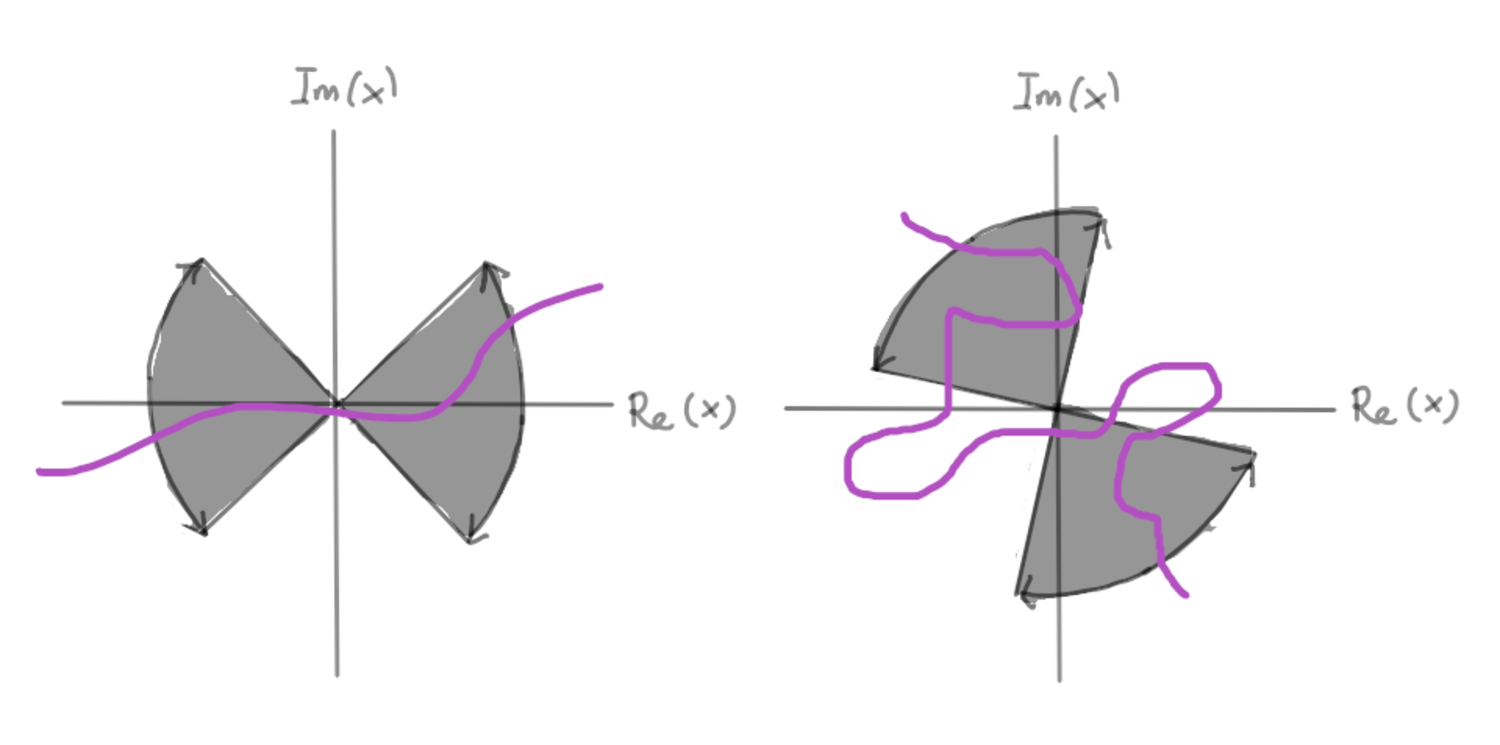
\includegraphics[width=.9\linewidth]{stokes1.pdf}
\captionof{figure}{Example of Stokes wedges in the complex plane. The configuration of the wedges varies depending on the problem at hand. Infinitely many possible integration contours are allowed to be used in order to solve the Schr\"{o}dinger equation for the Hamiltonians in equation \ref{eq:3.1}. But it is required that the endpoints of the integration contour must remain within the stokes wedges. The integration contour must be continuous but it need not be smooth and may even cross itself~\cite{PTsymmetricQM}. }
\label{fig:stokes1}
\end{Figure}
Stokes wedges must be non-adjacent in order to describe the boundary conditions of a valid coordinate-space eigenvalue problem. If the wedges are adjacent they would not represent a continuous region within the same Riemann sheet.
Determining the locations of Stokes wedges does not require that we solve the differential equation exactly but it can be done using complex asymptotic approximations~\cite{PTsymmetricQM}. One of such methods is the WKB approximation. 

\subsection{Complex WKB approximation}\label{WKB}
The WKB method works only for the eigenvalue problems with $\epsilon \geq 0$ because the sub-dominant eigenfunctions vanish exponentially in two \emph{Stokes wedges} in the complex x-plane~\cite{PTsymmetricQM}. The approximate solutions will contain either growing or decaying exponential terms. The nomenclature of the solutions depends on these exponential terms. Solutions are called either dominant or sub-dominant depending on these growing or decaying exponential terms respectively. 

The \emph{Stokes wedges} for the Hamiltonians in \ref{eq:3.1} are always centred about the origin of the complex x-plane. Their angular orientation of these wedges in the complex x-plane can be described by the argument of the complex variable $x = re^{i\theta}$~\cite{Scatteringoff}.

The limits of integration used in the WKB technique are analogous to classical turning points. i.e. the total energy of the system obeys the equation $E = x^2 (ix)^{\epsilon}$ and this equation has many complex solutions. However, since we are interested in $E$ being real, we are concerned with what happens to two turning points that lie on the real axis at $\pm \sqrt{E}$ when $\epsilon = 0$ as $\epsilon$ increases~\cite{PTsymmetricQM, MakingSense}.
The form of the turning points I used to find the eigenvalues for \ref{eq:3.1} when $\epsilon>0$ are
\begin{align}
x_{-}& = 
E^{\frac{1}{\epsilon + 2}}
e^{i\theta_{-}}
&\mathrm{and}&
&x_{+} = E^{\frac{1}{\epsilon + 2}} e^{i\theta_{+}},
\end{align}
where the angles are respectively
\begin{align}
\theta_{-}& = \frac{4 + 3\epsilon}{4 + 2 \epsilon} \pi
&\mathrm{and}&
&\theta_{+} = - \frac{\epsilon}{4 + 2 \epsilon} \pi.
\end{align}
When $\epsilon$ increases from 0, the turning points move into the complex plane. Notice that these turning points are always symmetric respect to reflections along the imaginary axis. \textbf{This left-right reflection symmetry is the coordinate space realisation of \PT-symmetry}~\cite{PTsymmetricQM}.
As $\epsilon$ increases from 0, a logarithmic branch-point singularity appears at the origin, and as $\epsilon$ continues increasing in the positive direction, it is necessary to introduce a branch-cut running from the origin along the positive imaginary axis. In this cut plane the solutions to equation \ref{eq:3.1} when $\epsilon>0$ are analytic and singled-valued~\cite{PTsymmetricQM}.
\begin{Figure}
 \centering
 \includegraphics[width=0.75\linewidth]{Stokes_wedges.pdf}
 \captionof{figure}{4 copies of the complex x-plane, each with a branch cut on the positive-imaginary axes, from zero to imaginary infinity, and four distinct instances of \emph{Stokes wedges} (one red and one yellow to differentiate between them) changing as functions of the parameter $\epsilon$ in equation \ref{eq:3.1}. For the cases when $\epsilon > 0$ the opening angles of the sectors decrease and the sectors rotate downward (both changes are respective to the $\epsilon = 0$ case). If $\epsilon = 0$, the angular opening is equal to $\pi/2$ and are centred about the positive-real and the negative-real axis. For the cases of $\epsilon < 0$ the angular behaviour is opposite to the positive $\epsilon$ values. The wedges get wider and rotate upwards as $\epsilon$ decreases from zero. The changes, get more dramatic for decreasing $\epsilon$ values. In the case of $\epsilon = -1$ the wedges fuse into one along the logarithmic branch cut on the positive-imaginary line. We can describe the topology of this scenario as the logarithmic Riemann surface collapsing onto a single sheet. When this occurs, The spectrum becomes null, meaning that there are no eigenvalues at all~\cite{PTsymmetricQM}.}
\end{Figure}



\bibliographystyle{unsrturl_mod}
\bibliography{mybib}

\end{document}